\subsubsection{Gestão de unidades curriculares}

É na página de gestão de unidades curriculares que um utilizador pode inscrever-se, verificar se já foi aprovado, e até sair de uma unidade curricular.

Nesta página foi colocada uma caixa de pesquisa, que permite ao utilizador encontrar mais facilmente a unidade curricular a que pretende candidatar-se.

Ao listar uma unidade curricular, é apresentada informação relativa ao ano letivo, curso, instituição e responsável.\\ 

Na Figura~\ref{fig:student_subjects} pode ser consultada uma imagem demonstrativa da página desenvolvida.

\begin{figure}[H]
  \centering
  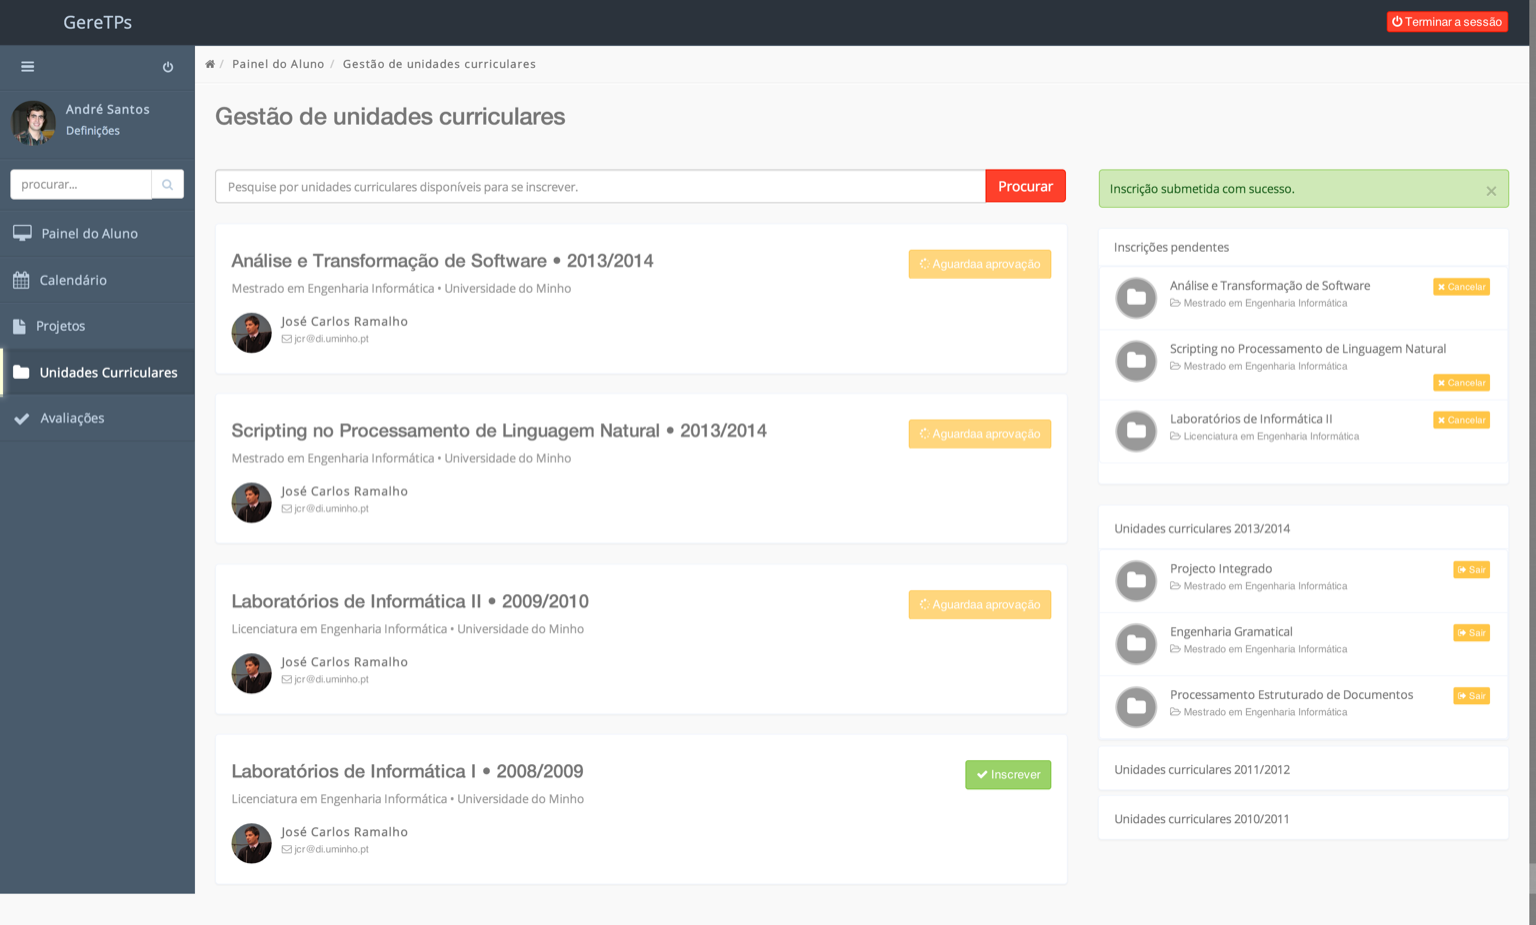
\includegraphics[width=1\textwidth,center]{images/implementacao/alunos/subjects}
  \caption{Página de gestão de unidades curriculares}
  \label{fig:student_subjects}
\end{figure}
